\documentclass{article}
\usepackage[UTF8]{ctex}
\usepackage{amsmath,mathtools,geometry,pgfplots,float,mathrsfs,caption,enumerate}
\pgfplotsset{compat=1.15}
\usetikzlibrary{arrows}
\geometry{scale=0.7}

\title{\vspace*{-1em}每日一题(17.2)\\{\fangsong\Large \hspace*{10em}——三角形中的两个模型}}
\author{\kaishu 程昊一}
\date{2022年5月18日}

\begin{document}
\maketitle
\begin{enumerate}
	\renewcommand{\labelenumi}{\textbf{\theenumi. }}
	\item {\heiti (婆罗摩笈多模型)}如图, $\triangle A_1OB_1$与$\triangle A_2OB_2$为等腰直角三角形, $\angle A_1OB_1=\angle A_2OB_2=90^\circ$, $H$, $M$分别为$A_1A_2$, $B_1B_2$上的点, 满足$H$, $O$, $M$共线. 
	\begin{enumerate}[(1) ]
		\item 求证: $\mathrm{S}_{\triangle A_1OA_2}=\mathrm{S}_{\triangle B_1OB_2}$; 
		\item 求证: 若$OH\perp A_1A_2$, 则$M$为$B_1B_2$中点; 反之亦然; 
		\item 求证: 若$OH\perp A_1A_2$, 则$A_1A_2=2OM$.
		\item 求证: $A_1A_2^2+B_1B_2^2=A_1B_1^2+A_2B_2^2$;
		\item 求$\left(\mathrm{S}_{\text{四边形}A_1A_2B_1B_2}\right)_{\mathrm{max}}$.
	\end{enumerate}
	\begin{figure}[H]
		\flushright
		\vspace*{-2cm}
		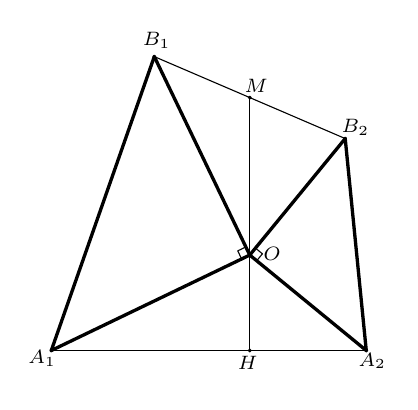
\begin{tikzpicture}[line cap=round,line join=round,>=triangle 45,x=1.0cm,y=1.0cm]
			\clip(-0.3,-0.4) rectangle (4.3,4.1);
			\draw[line width=0.4pt] (2.470896266869284,1.3152003682082873) -- (2.3678817635038083,1.2656563556511442) -- (2.417425776060951,1.1626418522856683) -- (2.520440279426427,1.2121858648428114) -- cycle; 
			\draw[line width=0.4pt] (2.608862765639377,1.1397423626095629) -- (2.6813062678726256,1.2281648488225128) -- (2.5928837816596757,1.3006083510557613) -- (2.520440279426427,1.2121858648428114) -- cycle; 
			\draw [line width=1.2pt] (0.,0.)-- (2.520440279426427,1.2121858648428114);
			\draw [line width=1.2pt] (2.520440279426427,1.2121858648428114)-- (1.308254414583616,3.732626144269238);
			\draw [line width=1.2pt] (1.308254414583616,3.732626144269238)-- (0.,0.);
			\draw [line width=1.2pt] (2.520440279426427,1.2121858648428114)-- (4.,0.);
			\draw [line width=1.2pt] (2.520440279426427,1.2121858648428114)-- (3.732626144269238,2.6917455854163843);
			\draw [line width=1.2pt] (3.732626144269238,2.6917455854163843)-- (4.,0.);
			\draw [line width=0.4pt] (1.308254414583616,3.732626144269238)-- (3.732626144269238,2.6917455854163843);
			\draw [line width=0.4pt] (4.,0.)-- (0.,0.);
			\draw [line width=0.4pt] (2.520440279426427,0.)-- (2.520440279426427,3.2121858648428114);
			\begin{scriptsize}
				\draw [fill=black] (0.,0.) circle (0.5pt);
				\draw[color=black] (-0.11573787956352835,-0.10444021296545353) node {$A_1$};
				\draw [fill=black] (2.520440279426427,1.2121858648428114) circle (0.5pt);
				\draw[color=black] (2.8051880246529043,1.229235357795899) node {$O$};
				\draw [fill=black] (1.308254414583616,3.732626144269238) circle (0.5pt);
				\draw[color=black] (1.3391809249033997,3.9370009105537966) node {$B_1$};
				\draw [fill=black] (4.,0.) circle (0.5pt);
				\draw[color=black] (4.076583712567102,-0.13138315378891519) node {$A_2$};
				\draw [fill=black] (3.732626144269238,2.6917455854163843) circle (0.5pt);
				\draw[color=black] (3.8610401859794083,2.8377289249565605) node {$B_2$};
				\draw [fill=black] (2.520440279426427,0.) circle (0.5pt);
				\draw[color=black] (2.4950330862299035,-0.16102038869472302) node {$H$};
				\draw [fill=black] (2.520440279426427,3.2121858648428114) circle (0.5pt);
				\draw[color=black] (2.6028048495237504,3.363116271014063) node {$M$};
			\end{scriptsize}
		\end{tikzpicture}
	\end{figure}
	%---%
	\item {\heiti (逆相似模型)}如图, 在$\triangle ABC$的边$AB, AC$上向外作直角三角形$\triangle APB$与$\triangle AQC$, 使得$\angle APB=\angle AQC=90^\circ$, $\angle PAB=\angle QAC$. 若$M$为$BC$中点, 求证: $PM=QM$.
	\begin{figure}[H]
		\flushright
		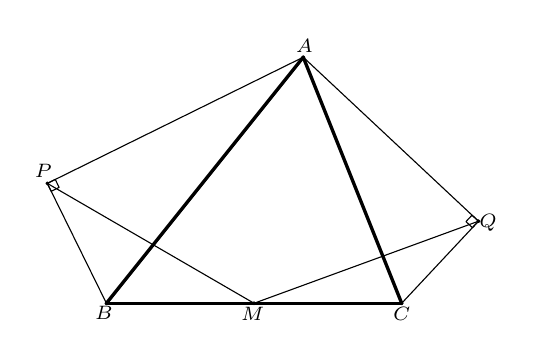
\begin{tikzpicture}[line cap=round,line join=round,>=triangle 45,x=1.25cm,y=1.25cm]
			\clip(-0.8,-0.3) rectangle (4.1,2.8);
			\draw[line width=0.4pt] (-0.5606754252947079,1.1372502648273293) -- (-0.4799777947037017,1.1770349804270723) -- (-0.5197625103034447,1.2577326110180784) -- (-0.6004601408944509,1.2179478954183356) -- cycle; 
			\draw[line width=0.4pt] (3.714665908758339,0.8953236860851223) -- (3.653188055352743,0.8296319459727233) -- (3.718879795465142,0.7681540925671271) -- (3.780357648870738,0.8338458326795261) -- cycle; 
			\draw [line width=1.2pt] (2.,2.5)-- (0.,0.);
			\draw [line width=1.2pt] (2.,2.5)-- (3.,0.);
			\draw [line width=0.4pt] (0.,0.)-- (-0.6004601408944509,1.2179478954183356);
			\draw [line width=0.4pt] (-0.6004601408944509,1.2179478954183356)-- (2.,2.5);
			\draw [line width=0.4pt] (2.,2.5)-- (3.780357648870738,0.8338458326795261);
			\draw [line width=0.4pt] (3.780357648870738,0.8338458326795261)-- (3.,0.);
			\draw [line width=1.2pt] (0.,0.)-- (3.,0.);
			\draw [line width=0.4pt] (-0.6004601408944509,1.2179478954183356)-- (1.5,0.);
			\draw [line width=0.4pt] (1.5,0.)-- (3.780357648870738,0.8338458326795261);
			\begin{scriptsize}
				\draw [fill=black] (2.,2.5) circle (0.5pt);
				\draw[color=black] (2.011866102482387,2.620078950268126) node {$A$};
				\draw [fill=black] (0.,0.) circle (0.5pt);
				\draw[color=black] (-0.023964136834665015,-0.09860268181986004) node {$B$};
				\draw [fill=black] (3.,0.) circle (0.5pt);
				\draw[color=black] (3.000092031150873,-0.10284399481843723) node {$C$};
				\draw [fill=black] (-0.6004601408944509,1.2179478954183356) circle (0.5pt);
				\draw[color=black] (-0.6389545216283579,1.3476850506949656) node {$P$};
				\draw [fill=black] (3.780357648870738,0.8338458326795261) circle (0.5pt);
				\draw[color=black] (3.8780438218563518,0.8217622388713928) node {$Q$};
				\draw [fill=black] (1.5,0.) circle (0.5pt);
				\draw[color=black] (1.4859432906588153,-0.11132662081559164) node {$M$};
			\end{scriptsize}
		\end{tikzpicture}
	\end{figure}
\end{enumerate}
\end{document}